%\title{LaTeX Portrait Poster Template}
%%%%%%%%%%%%%%%%%%%%%%%%%%%%%%%%%%%%%%%%%
% a0poster Portrait Poster
% LaTeX Template
% Version 1.0 (22/06/13)
%
% The a0poster class was created by:
% Gerlinde Kettl and Matthias Weiser (tex@kettl.de)
% 
% This template has been downloaded from:
% http://www.LaTeXTemplates.com
%
% License:
% CC BY-NC-SA 3.0 (http://creativecommons.org/licenses/by-nc-sa/3.0/)
%
%%%%%%%%%%%%%%%%%%%%%%%%%%%%%%%%%%%%%%%%%

%----------------------------------------------------------------------------------------
%	PACKAGES AND OTHER DOCUMENT CONFIGURATIONS
%----------------------------------------------------------------------------------------

\documentclass[a0,portrait]{a0poster}

\usepackage{multicol} % This is so we can have multiple columns of text side-by-side
\columnsep=100pt % This is the amount of white space between the columns in the poster
\columnseprule=3pt % This is the thickness of the black line between the columns in the poster

\usepackage[svgnames]{xcolor} % Specify colors by their 'svgnames', for a full list of all colors available see here: http://www.latextemplates.com/svgnames-colors

\usepackage{times} % Use the times font
%\usepackage{palatino} % Uncomment to use the Palatino font

\usepackage{graphicx} % Required for including images
\graphicspath{{figures/}} % Location of the graphics files
\usepackage{booktabs} % Top and bottom rules for table
\usepackage[font=small,labelfont=bf]{caption} % Required for specifying captions to tables and figures
\usepackage{amsfonts, amsmath, amsthm, amssymb} % For math fonts, symbols and environments
\usepackage{wrapfig} % Allows wrapping text around tables and figures
\usepackage{hyperref}

\begin{document}

%----------------------------------------------------------------------------------------
%	POSTER HEADER 
%----------------------------------------------------------------------------------------

% The header is divided into two boxes:
% The first is 75% wide and houses the title, subtitle, names, university/organization and contact information
% The second is 25% wide and houses a logo for your university/organization or a photo of you
% The widths of these boxes can be easily edited to accommodate your content as you see fit

\begin{minipage}[b]{0.65\linewidth}
\veryHuge \color{NavyBlue} \verb|$ whoami| \color{Black}\\ % Title
\Huge\textit{An Exploration of a participant of SGN 2017}\\[2cm] % Subtitle
\huge \textbf{Hyun-Hwan Jeong}\\[0.5cm] % Author(s)
\Large Department of Molecular Human Genetics, Baylor College of Medicine\\[0.2cm] % University/organization
\Large Jan and Dan Duncan Neurological Research Institute, Texas Children's Hospital\\[0.2cm] % University/organization
\Large \texttt{hyun-hwan.jeong@bcm.edu} \\
\end{minipage}
%
\begin{minipage}[b]{0.25\linewidth}

\includegraphics[width=20cm]{logo.pdf}\\
\end{minipage}

\vspace{1cm} % A bit of extra whitespace between the header and poster content

%----------------------------------------------------------------------------------------

\begin{multicols}{2} % This is how many columns your poster will be broken into, a portrait poster is generally split into 2 columns

%----------------------------------------------------------------------------------------
%	ABSTRACT
%----------------------------------------------------------------------------------------

\color{Black} % Navy color for the abstract

\section*{A Brief Introduction}

I, Hyun-Hwan has started majoring in Computer Science since 2003 and have got my B.S. degree in 2007. During the undergraduate program, I was an enthusiastic student for studying computational algorithms and got several awards from computer programming/algorithm competition like ACM-ICPC(ACM International Collegiate Programming Contest
) and Topcoder. 
In my M.S. between 2007 and 2009, I studied two topics on SNP genotype data analysis. The first topic was about developing an algorithm to detect high-order epistatic interaction and the second was about the application of a heuristic algorithm for imputation of SNP genotype data. I started my Ph.D. program in 2009 once I got the M.S. degree.
During the Ph.D. studies, I highly focused on the development of integrative network analysis framework for multiple omics data using information-theoretic measure. I have received the Ph.D. degree in computer science in August 2015 and started postdoctoral associate position of Dr. Zhandong Liu's lab at Baylor College of Medicine, and co-mentored by Dr. Huda Zoghbi, since September 2015. 
Until now, I have nine peer-reviewed publications in Bioinformatics field on various topics and have five system biology papers among the publications. 

I am working on the development of quantification and statistical analysis pipeline for high-throughput screening data from neurological disorder studies to identify primary genetic modifiers of pathogenic proteins of the neurological disorders. 
I am also studying on developing an integrative network algorithm to improve the identification of various sources. I expect this will help to increase the reliability of results from the pipeline and can detect novel modifier candidates, which are not identified primary analysis. 

\section*{Personal Information}

\begin{itemize}
\item Born: July 6th, 1984 Seoul, South Korea
\item Nationality: South Korea
\item Residence: Houston, Texas, USA
\item Occupation: Postdoctoral Associate (mentor: Zhandong Liu \& Huda Zoghbi)
\item Research areas: Computer Science, Bioinformatics, and Biomedical informatics.
\item{Education}
  \begin{itemize}
  	\item 2015, \textbf{Ph.D}. in Computer Science and Engineering, Ajou University, South Korea
    	\begin{itemize}
          \item Doctoral Advisor: Kyubum Wee \& Kyung-Ah Sohn, Ajou University
          \item Thesis: Integrative network analysis framework for multiple omics data using information-theoretic measure
         \end{itemize}
  	\item 2009,
    \textbf{M.Eng.} in Information and Communication Technology, Ajou University, South Korea
  	\item 2007, Information and Computer Engineering, Ajou University, South Korea
  \end{itemize}
  
\item Personality: INTJ PERSONALITY (``THE ARCHITECT'')
	\begin{itemize} 
    	\item source: \url{https://www.16personalities.com/intj-personality}
    \end{itemize}
\end{itemize}

\section*{More (Private) Personal Information}

\subsection*{Family}

\begin{center}\vspace{0.5cm}
\includegraphics[width=0.75\linewidth]{photo.pdf}
\captionof{figure}{Photos of my family. Seon Young and I have been married since 2016, and these lovely two cats (Mina and Emma, 2 years and 1 year old) were adopted in 2016.}
\end{center}

\subsection*{Hobby and Interest}

\begin{center}\vspace{0.5cm}
\includegraphics[width=0.75\linewidth]{hobby.pdf}
\captionof{figure}{
I also love to watch various sports games. Especially, I am a big fan of League of legends, and
I went to see Semi-final of World 2014 which held in Seoul, South Korea. I also enjoy to watch American football games, too.
I also love Music, and I did gigs as a DJ in some small parties.}
\end{center}

\section*{My scholar network}

\begin{center}\vspace{0.5cm}
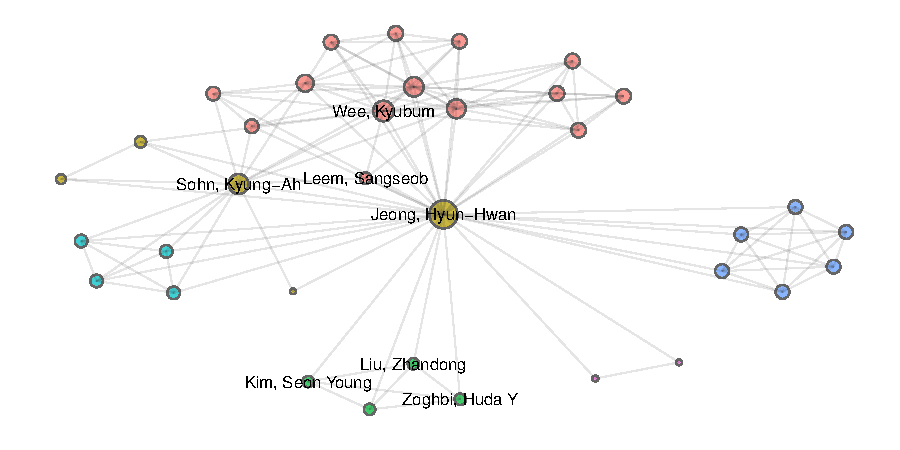
\includegraphics[width=0.5\linewidth]{network.pdf}
\captionof{figure}{My scholar network. The nodes represent people who published at least one paper with me, and the edges represents the connected people were co-authors.}
\end{center}

\section*{Research Highlights}

\subsection*{Integrative network analysis framework for multiple omics data
using information-theoretic measure (2015)}

\begin{center}\vspace{0.5cm}
\includegraphics[width=0.65\linewidth]{mina.pdf}
\captionof{figure}{(a) An workflow illustration of MINA, an integrative network analysis framework for multiple omics data.
 (b) Examples of the applications of MINA in \cite{jeong2015integrative} and \cite{jeong2015investigating}.
}
\end{center}\vspace{0.5cm}

\subsection*{CRISPRcloud: A secure cloud-based pipeline for CRISPR pooled screen deconvolution (2017)}

\begin{center}\vspace{0.5cm}
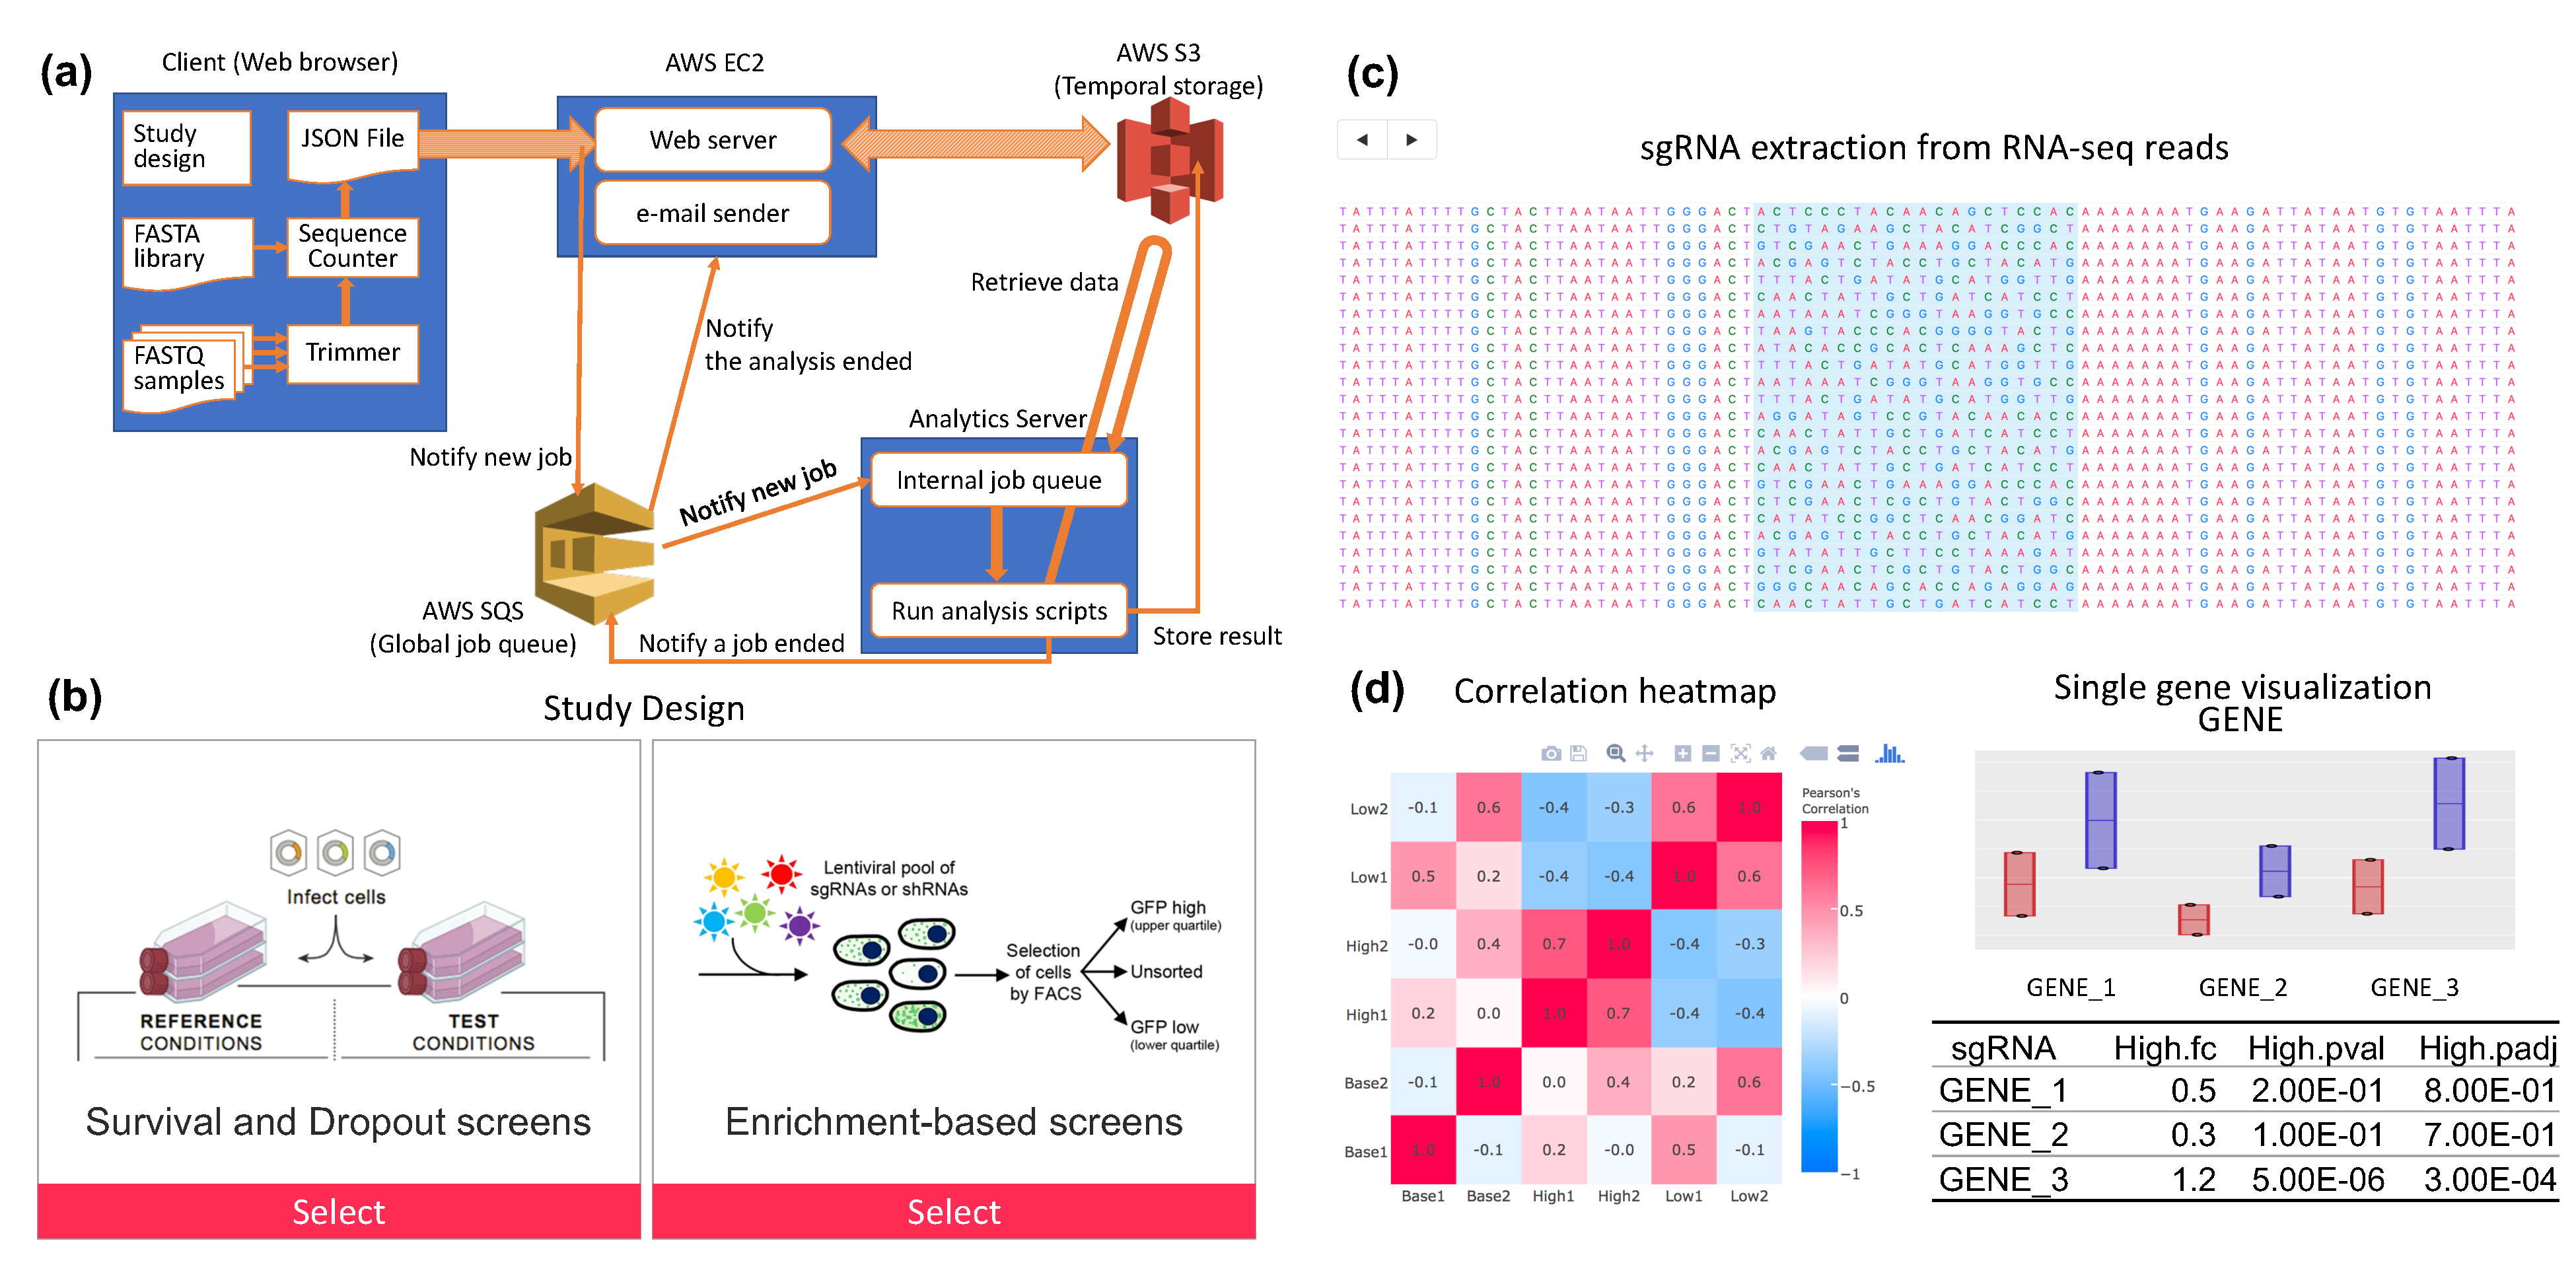
\includegraphics[width=0.65\linewidth]{crisprcloud.pdf}
\captionof{figure}{
This figure is from \cite{jeong2017crisprcloud} and shows details of the pipeline. 
(a) A detailed illustration of the pipeline of CRISPRcloud.
(b) A Screenshot of GUI to input user data in the CRISPRcloud website. 
(c) Another screenshot of GUI to pre-process raw seqeuncing files.
(d) An example of the visualized report.
}
\end{center}\vspace{0.5cm}

\section*{Further Information About Me?}

Please use those QR-code to reach the information! 

\begin{center}\vspace{0.5cm}
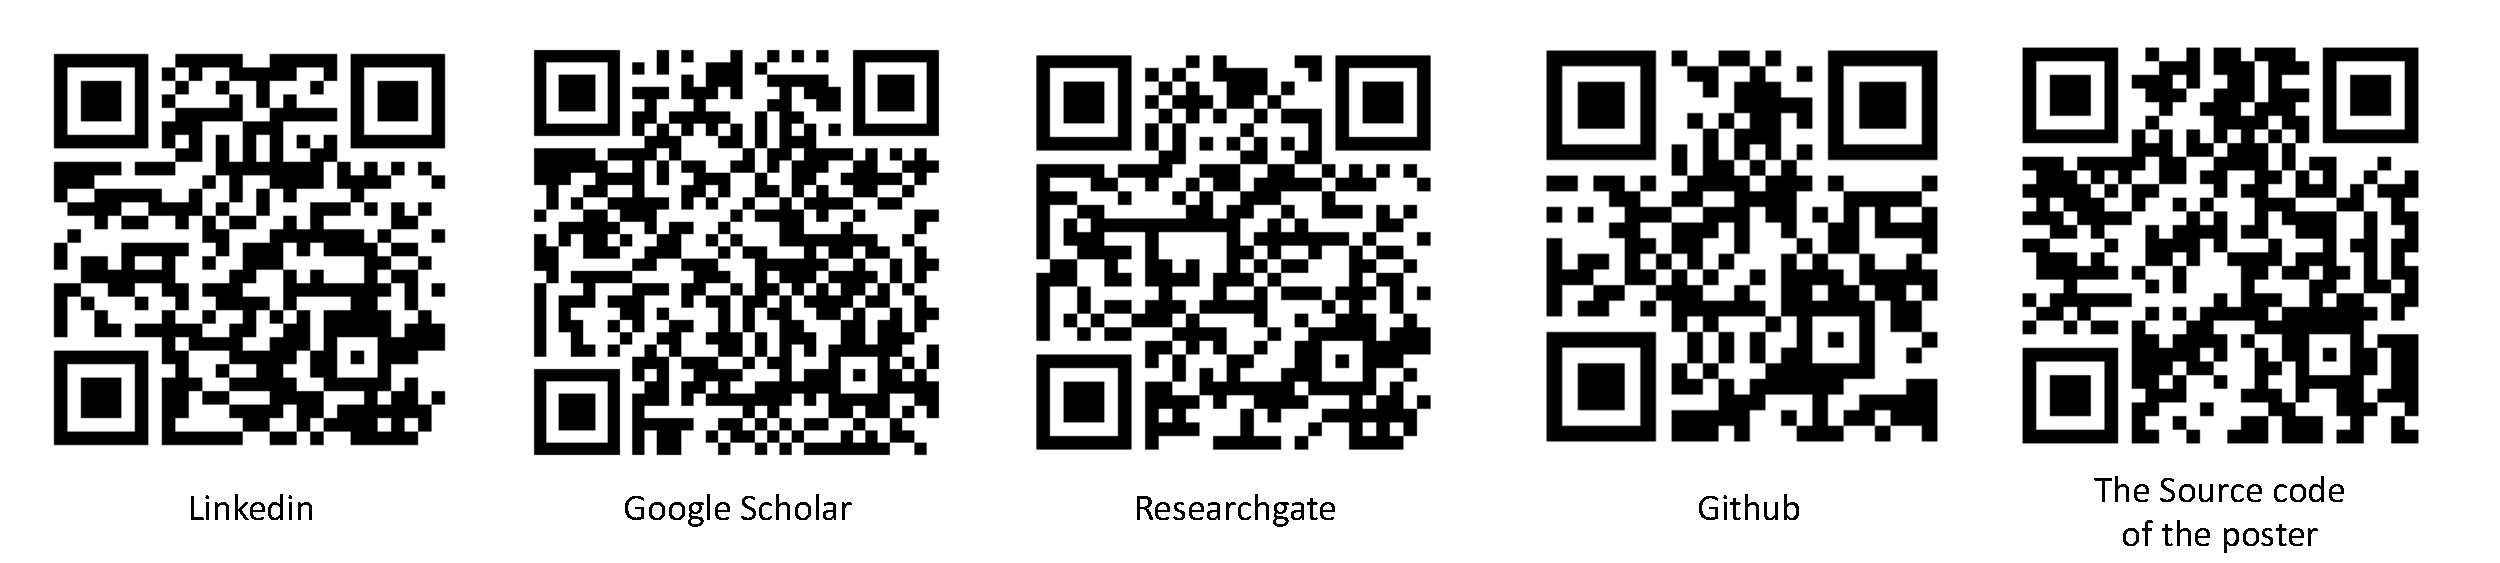
\includegraphics[width=0.8\linewidth]{qrcode.pdf}
\end{center}

\nocite{*} % Print all references regardless of whether they were cited in the poster or not
\bibliographystyle{plain} % Plain referencing style
\bibliography{sample} % Use the example bibliography file sample.bib

%----------------------------------------------------------------------------------------

\end{multicols}
\end{document}
